\documentclass[aspectratio=169]{../latex_main/tntbeamer}  % you can pass all options of the beamer class, e.g., 'handout' or 'aspectratio=43'
\usepackage{dsfont}
\usepackage{bm}
\usepackage[english]{babel}
\usepackage[T1]{fontenc}
%\usepackage[utf8]{inputenc}
\usepackage{graphicx}
\graphicspath{ {./figures/} }
\usepackage{algorithm}
\usepackage[ruled,vlined,algo2e,linesnumbered]{algorithm2e}
\usepackage{hyperref}
\usepackage{booktabs}
\usepackage{mathtools}

\usepackage{amsmath,amssymb}

\DeclareMathOperator*{\argmax}{arg\,max}
\DeclareMathOperator*{\argmin}{arg\,min}

\usepackage{amsbsy}
\newcommand{\vect}[1]{\bm{#1}}
%\newcommand{\vect}[1]{\boldsymbol{#1}}

\usepackage{pgfplots}
\pgfplotsset{compat=1.16}
\usepackage{tikz}
\usetikzlibrary{trees} 
\usetikzlibrary{shapes.geometric}
\usetikzlibrary{positioning,shapes,shadows,arrows,calc,mindmap}
\usetikzlibrary{positioning,fadings,through}
\usetikzlibrary{decorations.pathreplacing}
\usetikzlibrary{intersections}
\pgfdeclarelayer{background}
\pgfdeclarelayer{foreground}
\pgfsetlayers{background,main,foreground}
\tikzstyle{activity}=[rectangle, draw=black, rounded corners, text centered, text width=8em]
\tikzstyle{data}=[rectangle, draw=black, text centered, text width=8em]
\tikzstyle{myarrow}=[->, thick, draw=black]

% Define the layers to draw the diagram
\pgfdeclarelayer{background}
\pgfdeclarelayer{foreground}
\pgfsetlayers{background,main,foreground}

% Requires XeLaTeX or LuaLaTeX
%\usepackage{unicode-math}

\usepackage{fontspec}
%\setsansfont{Arial}
\setsansfont{RotisSansSerifStd}[ 
Path=../latex_main/fonts/,
Extension = .otf,
UprightFont = *-Regular,  % or *-Light
BoldFont = *-ExtraBold,  % or *-Bold
ItalicFont = *-Italic
]
\setmonofont{Cascadia Mono}[
Scale=0.8
]

% scale factor adapted; mathrm font added (Benjamin Spitschan @TNT, 2021-06-01)
%\setmathfont[Scale=1.05]{Libertinus Math}
%\setmathrm[Scale=1.05]{Libertinus Math}

% other available math fonts are (not exhaustive)
% Latin Modern Math
% XITS Math
% Libertinus Math
% Asana Math
% Fira Math
% TeX Gyre Pagella Math
% TeX Gyre Bonum Math
% TeX Gyre Schola Math
% TeX Gyre Termes Math

% Literature References
\newcommand{\lit}[2]{\href{#2}{\footnotesize\color{black!60}[#1]}}

%%% Beamer Customization
%----------------------------------------------------------------------
% (Don't) Show sections in frame header. Options: 'sections', 'sections light', empty
\setbeamertemplate{headline}{empty}

% Add header logo for normal frames
\setheaderimage{
	% 
\includegraphics[height=\logoheight]{figures/TNT_darkv4.pdf}
	
\includegraphics[height=\logoheight]{../latex_main/figures/luh_logo_rgb_0_80_155.pdf}
	% 
\includegraphics[height=\logoheight]{figures/logo_tntluh.pdf}
}

% Header logo for title page
\settitleheaderimage{
	% 
\includegraphics[height=\logoheight]{figures/TNT_darkv4.pdf}
	
\includegraphics[height=\logoheight]{../latex_main/figures/luh_logo_rgb_0_80_155.pdf}
	% 
\includegraphics[height=\logoheight]{figures/logo_tntluh.pdf}
}

% Title page: tntdefault 
\setbeamertemplate{title page}[tntdefault]  % or luhstyle
% Add optional title image here
%\addtitlepageimagedefault{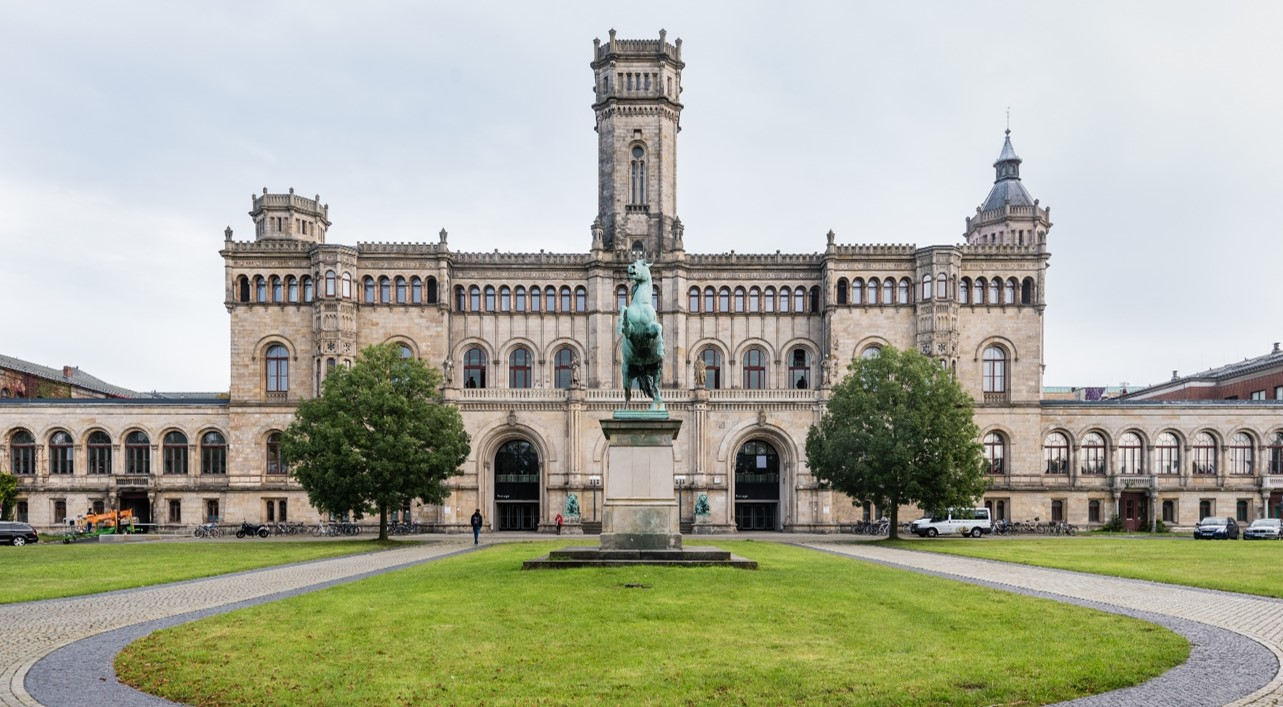
\includegraphics[width=0.65\textwidth]{figures/luh_default_presentation_title_image.jpg}}

% Title page: luhstyle
% \setbeamertemplate{title page}[luhstyle]
% % Add optional title image here
% \addtitlepageimage{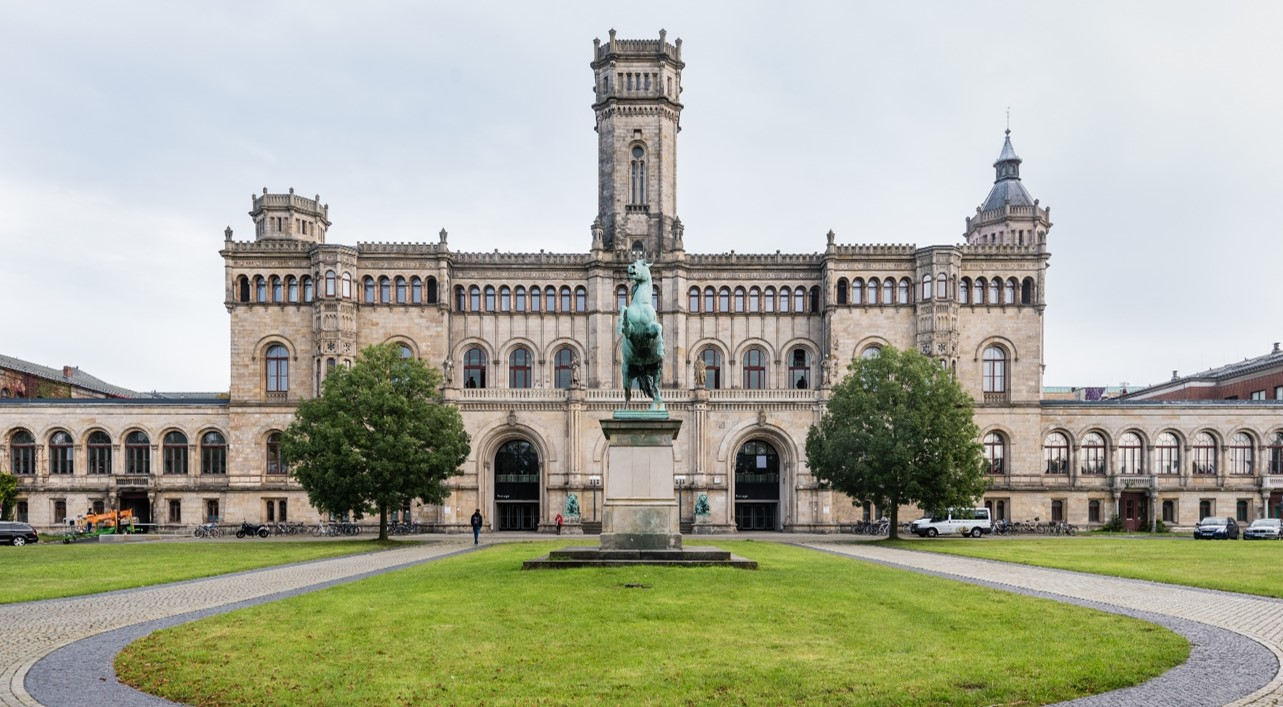
\includegraphics[width=0.75\textwidth]{figures/luh_default_presentation_title_image.jpg}}

\author[Abedjan \& Lindauer]{Ziawasch Abedjan \& Marius Lindauer\\[1em]
	
\includegraphics[height=\logoheight]{../latex_main/figures/luh_logo_rgb_0_80_155.pdf}\qquad
	
\includegraphics[height=\logoheight]{../latex_main/figures/DBIS_Kurzlogo.png}\qquad

\includegraphics[height=\logoheight]{../latex_main/figures/TNT_darkv4}\qquad

\includegraphics[height=\logoheight]{../latex_main/figures/L3S.jpg}	}
\date{Summer Term 2022; \hspace{0.5em} {
\includegraphics[height=1.5em]{../latex_main/figures/Cc-by-nc-sa_icon.svg.png}}; based on \href{https://ds100.org/fa21/}{[DS100]}
}


%%% Custom Packages
%----------------------------------------------------------------------
% Create dummy content
\usepackage{blindtext}

% Adds a frame with the current page layout. Just call \layout inside of a frame.
\usepackage{layout}


%%% Macros
%\renewcommand{\vec}[1]{\mathbf{#1}}
% \usepackage{bm}
%\let\vecb\bm

\title[Introduction]{DS: Decision Trees}
\subtitle{Basic Decision Tree Generation}

\graphicspath{ {./figure_tree/} }
%\institute{}


\begin{document}
	
	\maketitle
	\begin{frame}{Basic Decision Tree Generation}
	    \begin{figure}
	        \centering
	        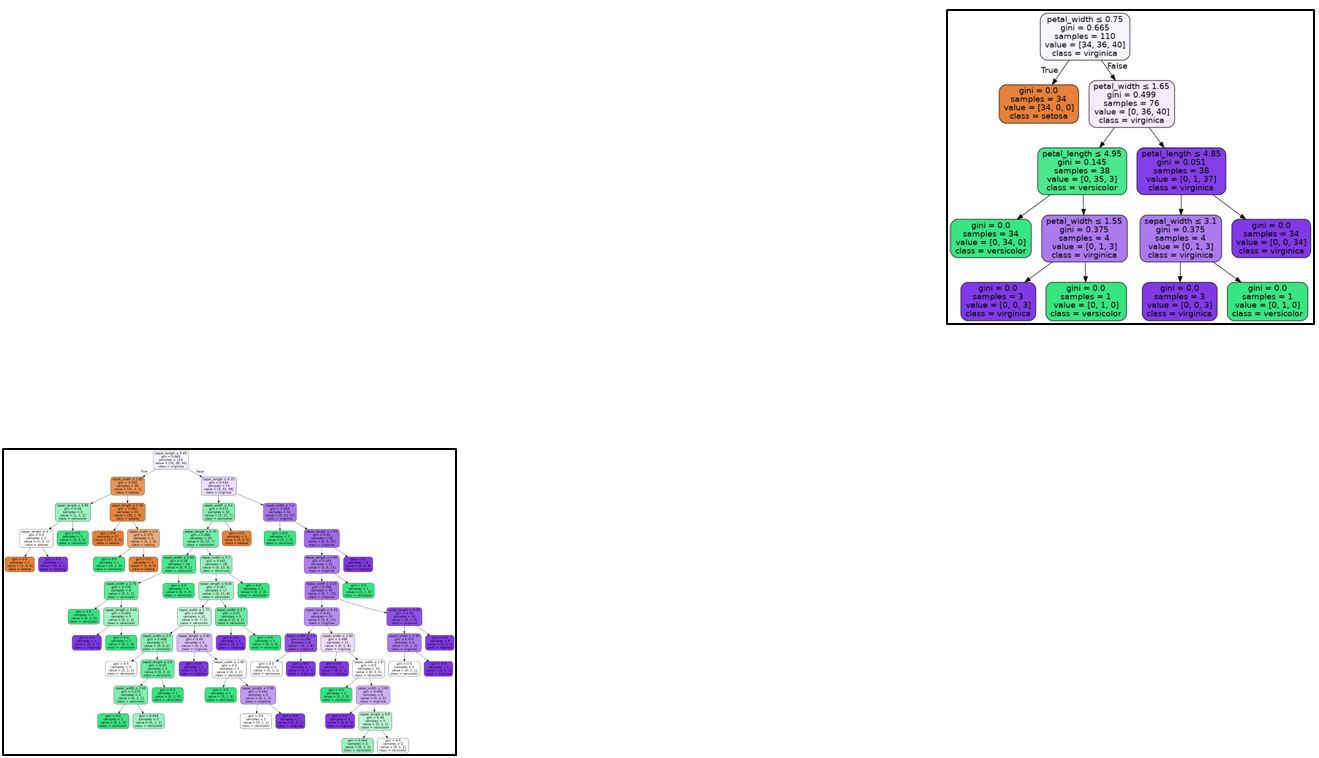
\includegraphics[scale=.3]{Bild40}
	    \end{figure}
	\end{frame}
	
	\begin{frame}{Decision Tree Generation}
	    Let’s discuss how decision trees are created from data\\
	    \bigskip
	    Traditional decision tree generation algorithm: 
	    \begin{itemize}
	        \item All of the data starts in the root node
	        \item Repeat until every node is either pure or unsplittable:
	        \begin{itemize}
	            \item Pick the best feature x and best split value $\beta$, e.g. x = petal\_length, $\beta$ = 2
	            \item Split data into two nodes, one where x < $\beta$, and one where x ≥ $\beta$
	        \end{itemize}
	    \end{itemize}
	    
Notes: 
\begin{itemize}
    \item A node that has only one class is called a “\alert{pure}” node.
    \item A node that has duplicate data that cannot be split is called “\alert{unsplittable}”.
\end{itemize}

	\end{frame}
	
	
	\begin{frame}{Defining a Best Feature}
	    Question: Which feature and split value is best?
	    \begin{itemize}
	        \item  Equivalently: Which horizontal or vertical line do we want to draw?
	    \end{itemize}
	    \begin{figure}
	        \centering
	        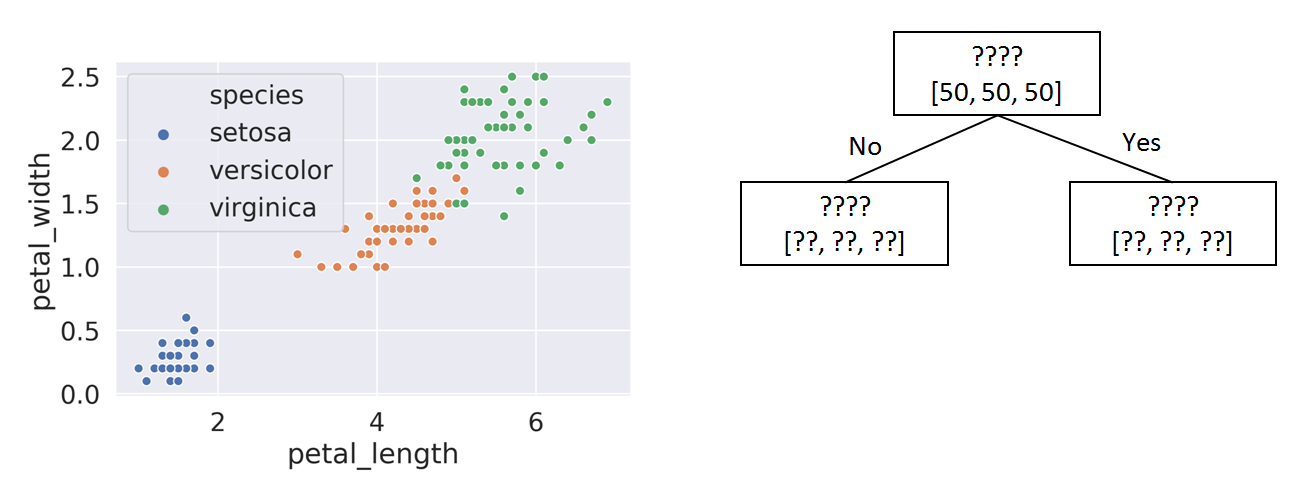
\includegraphics[scale=.4]{Bild41}
	    \end{figure}
	\end{frame}
	
	\begin{frame}{Defining a Best Feature}
	    Question: Which feature and split value is best?
	    \begin{itemize}
	        \item  Equivalently: Which horizontal or vertical line do we want to draw?
	    \end{itemize}
	    \begin{figure}
	        \centering
	        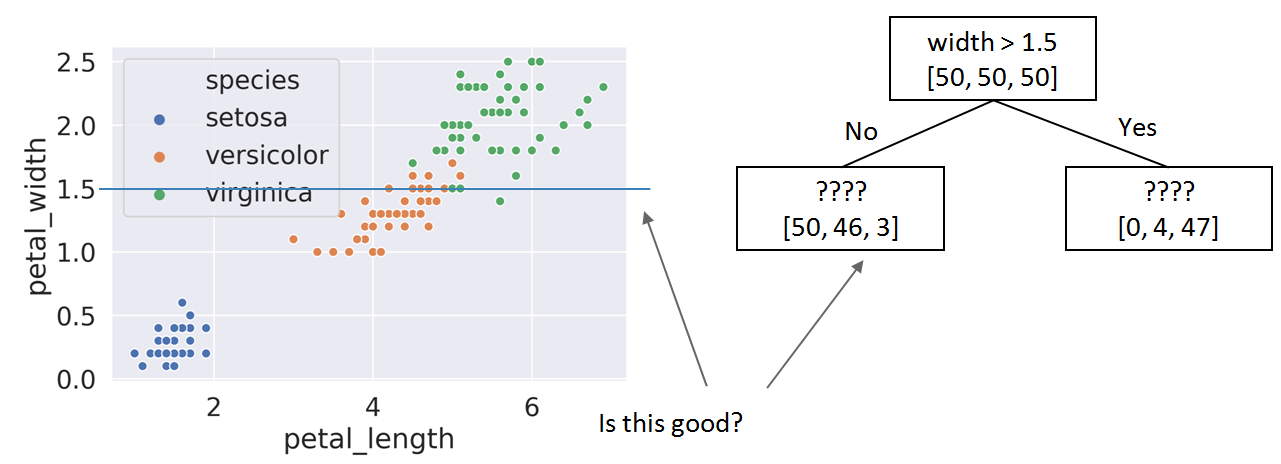
\includegraphics[scale=.4]{Bild42}
	    \end{figure}
	\end{frame}
	
	\begin{frame}{Defining a Best Feature}
	    Question: Which feature and split value is best?
	    \begin{itemize}
	        \item  Equivalently: Which horizontal or vertical line do we want to draw?
	    \end{itemize}
	    \begin{figure}
	        \centering
	        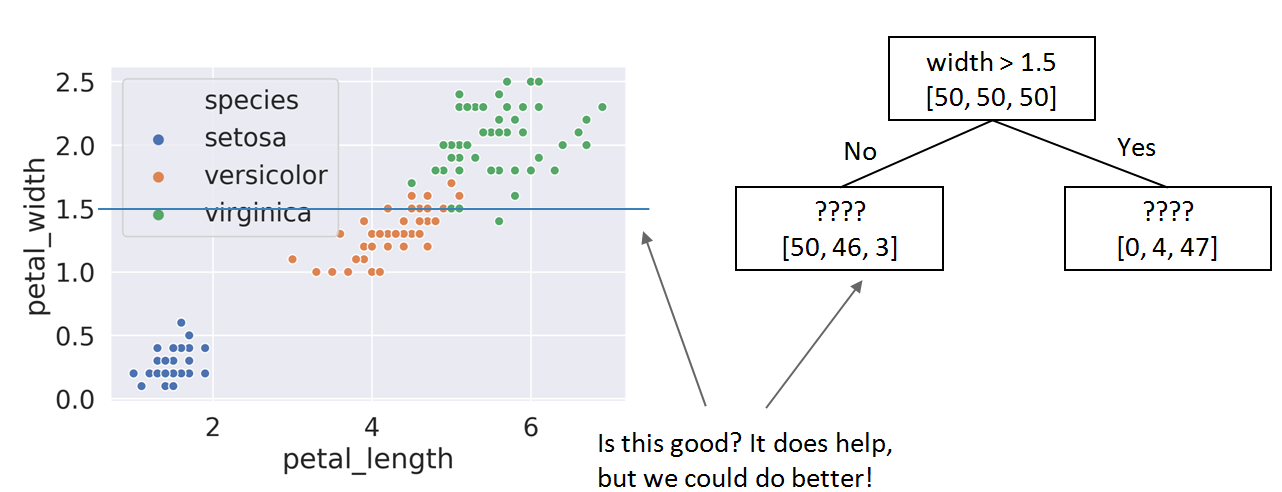
\includegraphics[scale=.4]{Bild43}
	    \end{figure}
	\end{frame}
	
	\begin{frame}{Defining a Best Feature}
	    Question: Which feature and split value is best?
	    \begin{itemize}
	        \item  Equivalently: Which horizontal or vertical line do we want to draw?
	    \end{itemize}
	    \begin{figure}
	        \centering
	        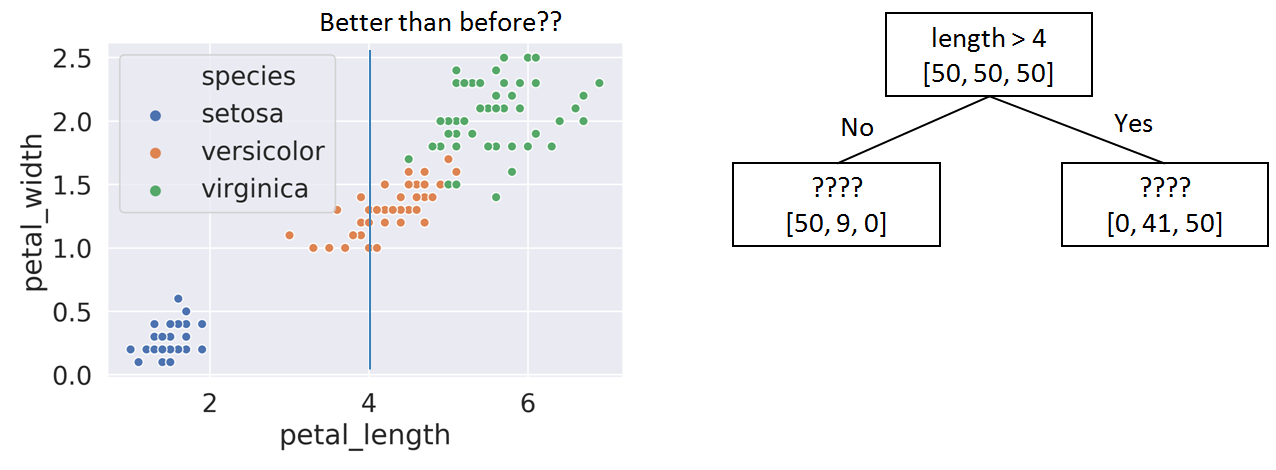
\includegraphics[scale=.4]{Bild44}
	    \end{figure}
	\end{frame}
	
	\begin{frame}{Defining a Best Feature}
	    Question: Which feature and split value is best?
	    \begin{itemize}
	        \item  Equivalently: Which horizontal or vertical line do we want to draw?
	    \end{itemize}
	    \begin{figure}
	        \centering
	        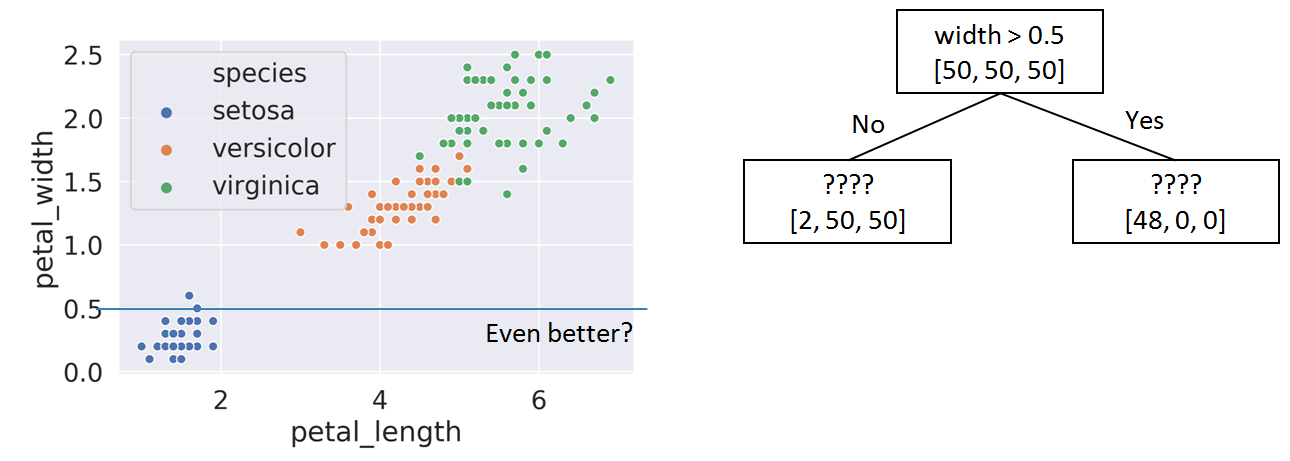
\includegraphics[scale=.4]{Bild45}
	    \end{figure}
	\end{frame}
	
	
	\begin{frame}{Defining a Best Feature}
	    Question: Which feature and split value is best?
	    \begin{itemize}
	        \item  Equivalently: Which horizontal or vertical line do we want to draw?
	    \end{itemize}
	    \alert{We need some sort of rigorous definition for a good split.}
	    \begin{figure}
	        \centering
	        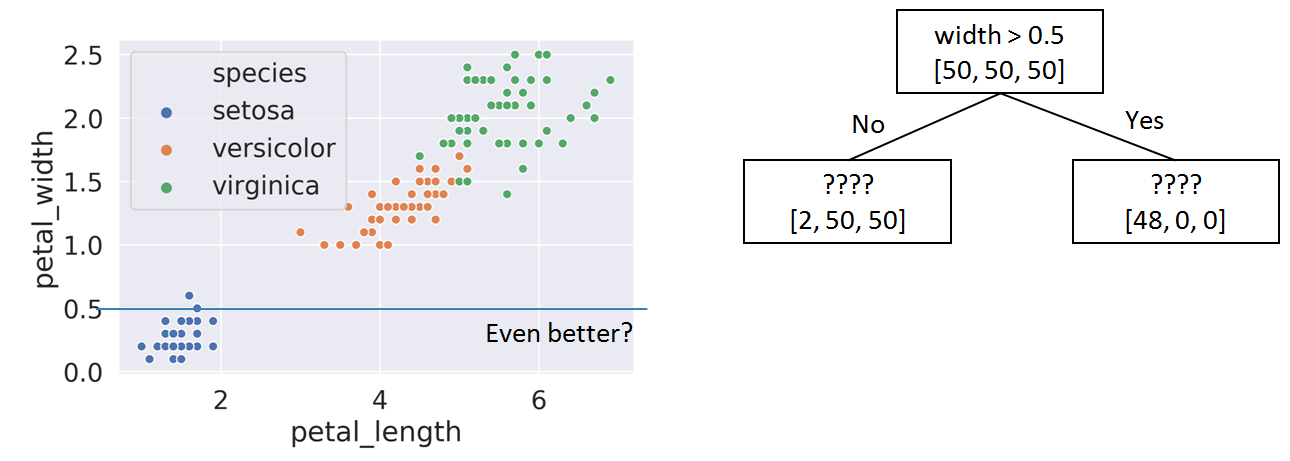
\includegraphics[scale=.4]{Bild45}
	    \end{figure}
	\end{frame}
	
	
	\begin{frame}{Defining a Best Feature}
	    Question: Which feature and split value is best?
	    \begin{itemize}
	        \item  Equivalently: Which horizontal or vertical line do we want to draw?
	    \end{itemize}
	   \alert{We need some sort of rigorous definition for a good split.}
	    \begin{figure}
	        \centering
	        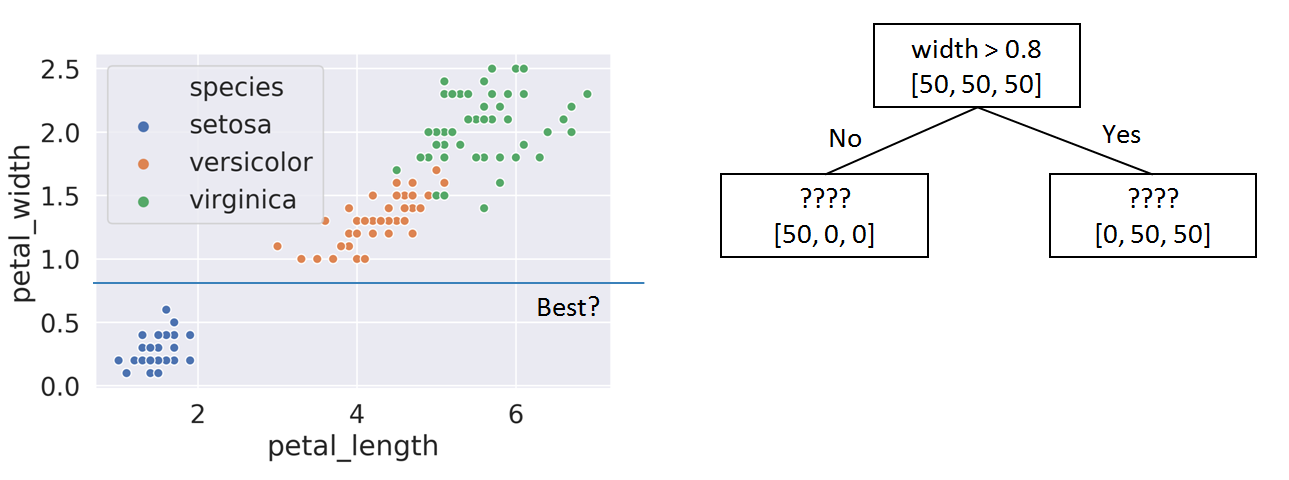
\includegraphics[scale=.4]{Bild46}
	    \end{figure}
	\end{frame}
	
	
	
	\begin{frame}{Node Entropy}
	
	    \vspace{-2em}
	    \begin{columns}
	        \begin{column}{.5\textwidth}
	        
	                Let $p_c$ the proportion of data points in a node with label C.\\
	                \bigskip
	                For example, for the node at the top of the decision tree, $p_0$ = 34/110 = 0.31,\\
                    $p_1$ = 36/110 = 0.33, and $p_2$ = 40/110 = 0.36\\
                    \bigskip
                    Define the entropy $S$ of a node as:
                    \begin{equation*}
                        S = -\sum\limits_c p_c\log_2p_c
                    \end{equation*}
                    For example, $S$ for the top node is:
                    $-0.31 \log_2  0.31 - 0.33 \log_2 0.33 - 0.36 \log_2 0.36 = 0.52 + 0.53 + 0.53 = 1.58$
                    
	        \end{column}
	        
	        \begin{column}{.5\textwidth}

	                    \centering
	                    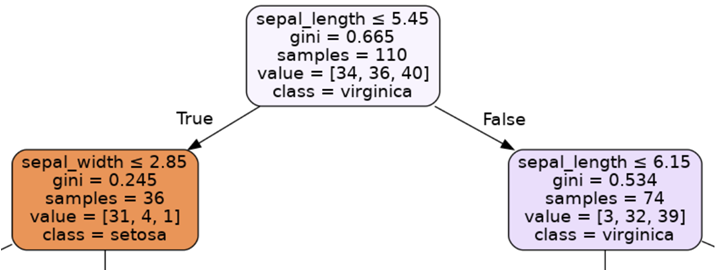
\includegraphics[scale=.5]{Bild47}
	                    
	        \end{column}
	    \end{columns}
	\end{frame}
	
	
% 	\begin{frame}{Test Your Understanding}
% 	    What is $p_0$?
% 	    \begin{figure}
%             \centering
%             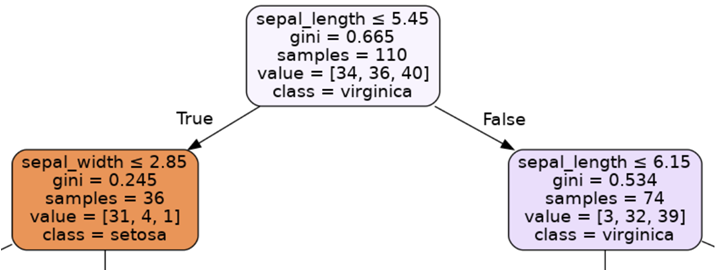
\includegraphics[scale=.5]{Bild47}
% 	   \end{figure}
% 	   What is the entropy of the node on the left with [31, 4, 1] in each class?
% 	   \begin{itemize}
% 	       \item Try writing out an expression, or try to compute an exact value
% 	   \end{itemize}
% 	   \begin{equation*}
%             S = -\sum\limits_c p_c\log_2p_c
%         \end{equation*}
% 	\end{frame}
	
	
% 	\begin{frame}{Test Your Understanding}
	
% 	    \vspace{-2em}
% 	    \begin{columns}
% 	        \begin{column}{.7\textwidth}
	            
% 	                What is the entropy of the node on the left with [31, 4, 1] in each class?
% 	                \begin{itemize}
% 	                    \item $p_0$ = 31/36 = 0.86, $p_1$ = 4/36 = 0.11, and $p_2$=1/36 = 0.028
% 	                    \item $S$ =  −0.86 log$_2$⁡0.86 
% 	                    \begin{itemize}
% 	                        \item 0.11 log$_2$⁡0.11 
% 	                        \item 0.028 log$_2$⁡0.028 = 0.68
% 	                    \end{itemize}
% 	                \end{itemize}
% 	                Define the entropy $S$ of a node as:
%                     \begin{equation*}
%                         S = -\sum\limits_c p_c\log_2p_c
%                     \end{equation*}
%                     Can think of entropy as how unpredictable a node is:
%                     \begin{itemize}
%                         \item Low entropy means more predictable 
%                         \item High entropy means more unpredictable
%                     \end{itemize}
                    
% 	        \end{column}
	        
% 	        \begin{column}{.3\textwidth}

% 	                    \centering
% 	                    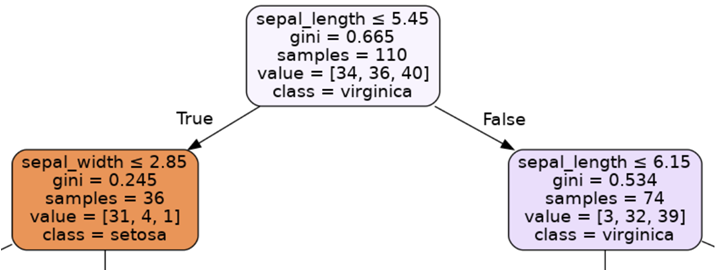
\includegraphics[scale=.35]{Bild47}
	                
% 	        \end{column}
% 	    \end{columns}
% 	\end{frame}
	
	
	\begin{frame}{Exploring Entropy}
	    \begin{columns}
	        \begin{column}{.7\textwidth}
	                Observations about entropy:
	                \begin{itemize}
	                    \item A node where all data are part of the \alert{same class} has zero entropy \\ $-1 \log_2 1 = 0$
	                    \item A node where data are \alert{evenly split between two classes} has
	                    entropy 1 \\$-0.5 \log_2{ 0.5} - 0.5\log_2{ 0.5}= 1$
	                    \item A node where data are \alert{evenly split between 3 classes} has entropy 1.58 \\$3 \cdot (-0.33 \log_2{ 0.33}) = 1.58$
	                    \item A node where data are \alert{evenly split into C classes} has entropy $\log_2{C}$ \\ 
	                    $C \cdot (-1 /C \log_2 1/C) = - \log_2 1/C = \log_2 C$
	                \end{itemize}
	        \end{column}
	        
	        \begin{column}{.3\textwidth}
	                \begin{figure}
	                    \centering
	                    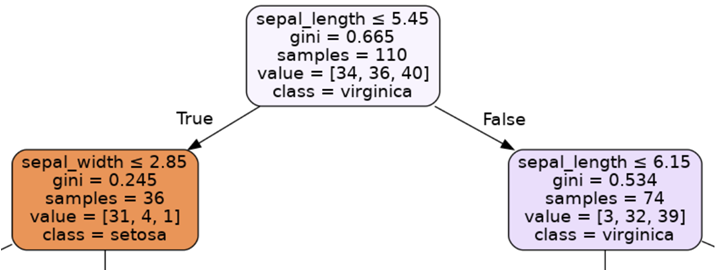
\includegraphics[scale=.35]{Bild47}
	                \end{figure}
	                \begin{equation*}
                          S = -\sum\limits_c p_c\log_2p_c
                    \end{equation*}
	                
	        \end{column}
	    \end{columns}
	\end{frame}
	
	
	\begin{frame}[c]{Weighted Entropy as a Loss Function}
	
	    \begin{itemize}
	        \item Idea: If there are more points in one of the leaf nodes, it should have a higher weight for the loss.
	        \item[$\leadsto$] We can use \alert{Weighted Entropy} as a loss function in helping us decide which split to take.
	        \item Suppose a given split results in two nodes $X_1$ and $X_2$ with $N_1$ and $N_2$ total samples each.\\ The loss of that split is given by:
	    \end{itemize}
	    
	    \begin{equation*}
	        \mathcal{L}=\frac{N_1S(X_1) + N_2S(X_2)}{N_1 + N_2}
	    \end{equation*}
	\end{frame}
	
	\begin{frame}{Defining a Best Feature}
	    Split choice \#1: width > 1.5. Compute entropy of child nodes:
	    \begin{itemize}
	        \item entropy([50, 46, 3]) = 1.16
	        \item entropy([4, 47]) = 0.4
	        \item Weighted loss: $99/150 \cdot 1.16 + 51/150 \cdot 0.4 = 0.9$
	    \end{itemize}
	    
	    \begin{figure}
	        \centering
	        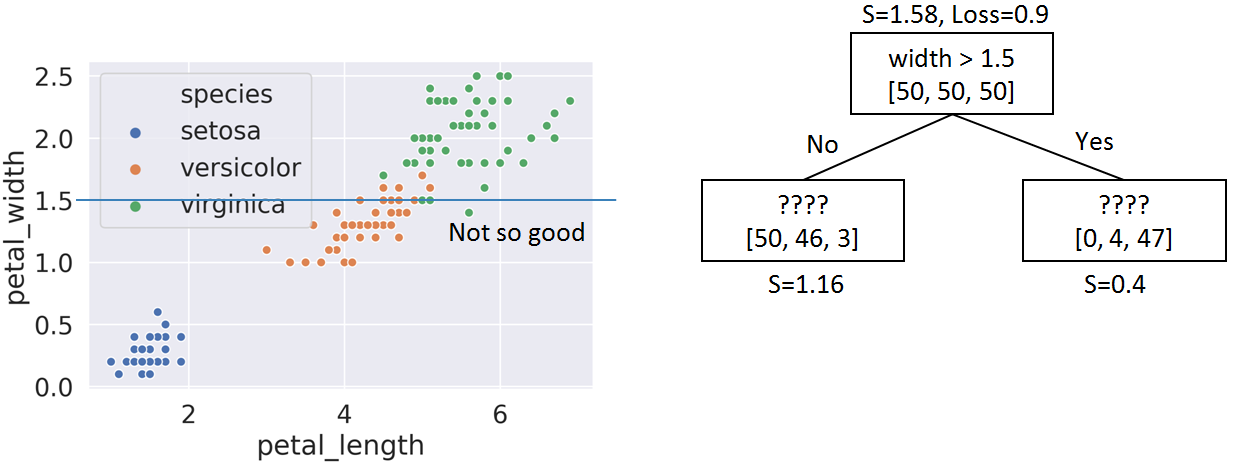
\includegraphics[scale=.4]{Bild48}
	    \end{figure}
	\end{frame}
	
	
	\begin{frame}{Defining a Best Feature}
	    Split choice \#2: length > 4. Compute entropy of child nodes:
	    \begin{itemize}
	        \item entropy([50, 9]) = 0.62
	        \item entropy([41, 50]) = 0.99
	        \item Weighted loss: 0.84: \alert{Better/smaller than split choice \#1!}
	    \end{itemize}
	    
	    \begin{figure}
	        \centering
	        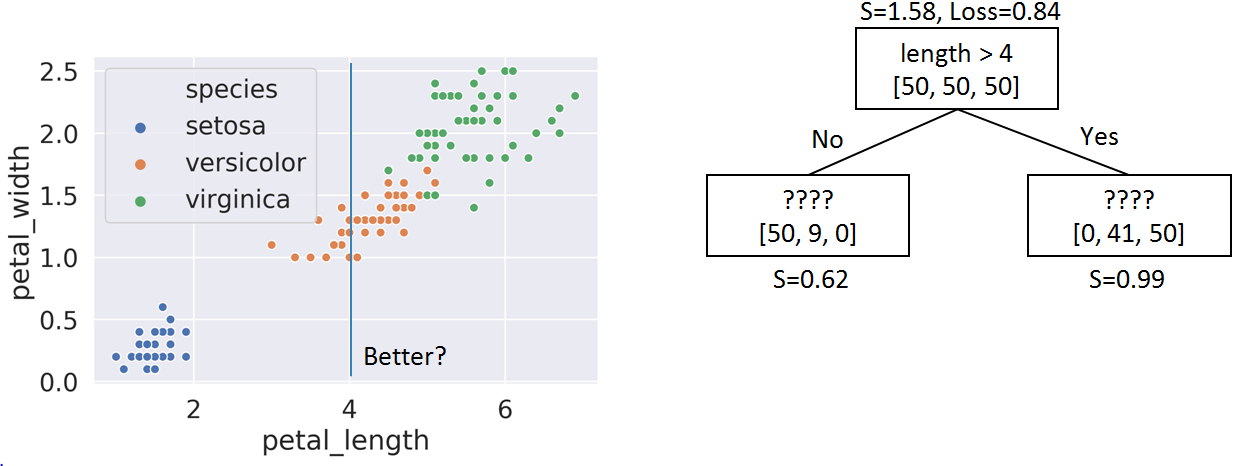
\includegraphics[scale=.4]{Bild49}
	    \end{figure}
	\end{frame}
	
	
	\begin{frame}{Defining a Best Feature}
	    Split choice \#3: width > 0.5. Compute entropy of child nodes:
	    \begin{itemize}
	        \item entropy([2, 50, 50]) = 1.12
	        \item entropy([48]) = 0
	        \item Weighted loss: 0.76: \alert{Lower than split choice \#2!}

	    \end{itemize}
	    
	    \begin{figure}
	        \centering
	        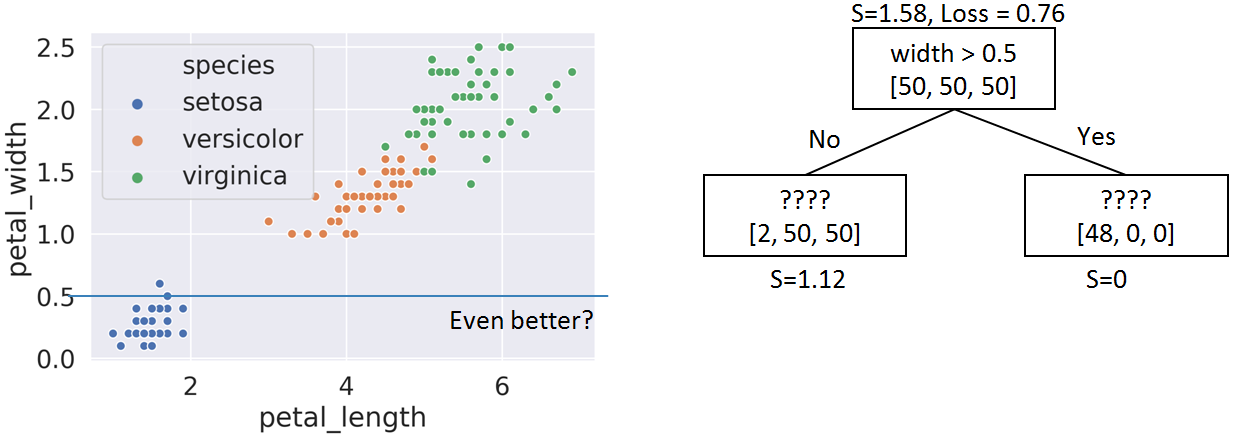
\includegraphics[scale=.4]{Bild50}
	    \end{figure}
	\end{frame}
	
	
	\begin{frame}{Defining a Best Feature}
 	    Split choice \#4: width > 0.9. Compute entropy of child nodes:
	    \begin{itemize}
	        \item entropy([50, 50]) = 1
	        \item entropy([50]) = 0
	        \item Weighted loss: 0.66: \alert{Lower than split choice \#3!}

	    \end{itemize}
	    
	    \begin{figure}
	        \centering
	        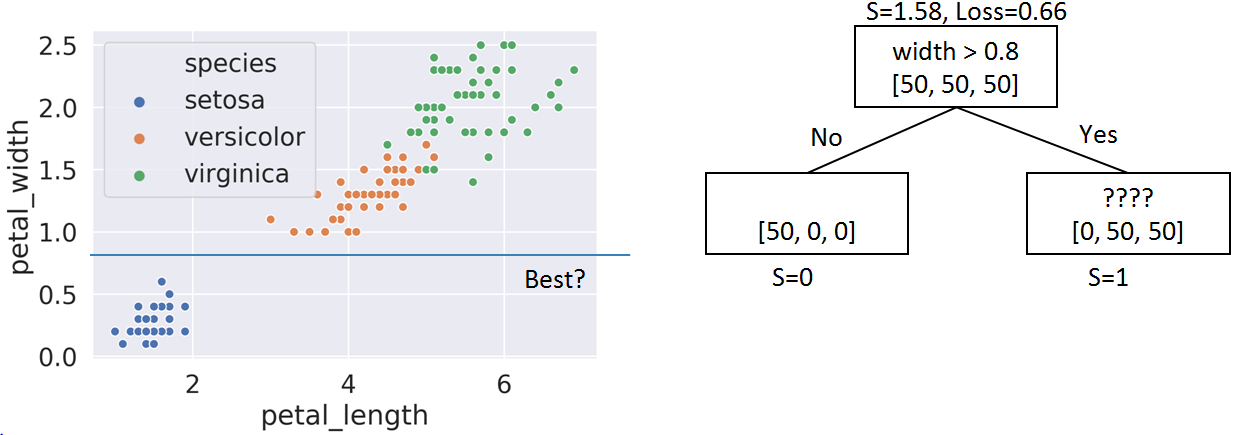
\includegraphics[scale=.4]{Bild51}
	    \end{figure}
	\end{frame}
	
	
	\begin{frame}[c]{Decision Tree Generation}
	    Traditional decision tree generation algorithm: 
	    \begin{itemize}
	        \item All of the data starts in the root node
	        \item Repeat until every node is either pure or unsplittable:
	        \begin{itemize}
	            \item Pick the best feature $f_i$ and split value $\beta$ such that the loss of the resulting split is minimized,\\ e.g. $f_i$ = petal\_width, $\beta$ = 0.8 has loss 0.66
	            \item Split data into two nodes, one where $x < \beta$ , and one where $x \geq \beta$ 
	        \end{itemize}
	    \end{itemize}

	\end{frame}
\end{document}